\tikzset{every picture/.style={line width=0.75pt}} %set default line width to 0.75pt        

\begin{tikzpicture}[x=0.75pt,y=0.75pt,yscale=-1,xscale=1]
%uncomment if require: \path (0,400); %set diagram left start at 0, and has height of 400

%Straight Lines [id:da2829187281066927] 
\draw [line width=5.25]    (98.42,50.08) -- (188,52.76) ;
\draw [shift={(196,53)}, rotate = 181.71] [fill={rgb, 255:red, 0; green, 0; blue, 0 }  ][line width=5.25]  [draw opacity=0] (29.47,-14.16) -- (0,0) -- (29.47,14.16) -- (19.57,0) -- cycle    ;

\draw  [color={rgb, 255:red, 214; green, 34; blue, 34 }  ,draw opacity=1 ][line width=5.25]  (344.29,34.58) -- (372.61,65.57)(372.57,34.46) -- (344.33,65.7) ;
%Straight Lines [id:da15738901895338753] 
\draw [line width=5.25]    (99.88,84.99) -- (231.56,137.06) ;
\draw [shift={(239,140)}, rotate = 201.57999999999998] [fill={rgb, 255:red, 0; green, 0; blue, 0 }  ][line width=5.25]  [draw opacity=0] (29.47,-14.16) -- (0,0) -- (29.47,14.16) -- (19.57,0) -- cycle    ;

%Straight Lines [id:da7632009543226708] 
\draw [line width=5.25]    (50.84,100.54) -- (50.84,164.45) ;
\draw [shift={(50.84,172.45)}, rotate = 270] [fill={rgb, 255:red, 0; green, 0; blue, 0 }  ][line width=5.25]  [draw opacity=0] (29.47,-14.16) -- (0,0) -- (29.47,14.16) -- (19.57,0) -- cycle    ;

\draw  [color={rgb, 255:red, 214; green, 34; blue, 34 }  ,draw opacity=1 ][line width=5.25]  (343.69,125.13) -- (372,156.12)(371.96,125.01) -- (343.72,156.24) ;
%Image [id:dp3582590935616692] 
\draw (50.84,52.29) node  {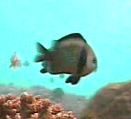
\includegraphics[width=56.75pt,height=58.19pt]{fish.png}};
%Straight Lines [id:da03584674957949119] 
\draw [color={rgb, 255:red, 43; green, 143; blue, 26 }  ,draw opacity=1 ][line width=4.5]    (107.77,220.31) -- (117.52,235.45) -- (135,208) ;



% Text Node
\draw (267.15,52.28) node [scale=0.7]  {$\begin{pmatrix}
	c_{1,1} & c_{1,2} & c_{1,3} & \dotsc  & c_{1,n}\\
	c_{2,1} & c_{2,2} & c_{2,3} & \dotsc  & c_{2,n}\\
	c_{3,1} & c_{3,2} & c_{3,3} & \dotsc  & c_{3,n}\\
	\vdots  & \vdots  & \vdots  & \ddots  & \vdots \\
	c_{n,1} & c_{n,2} & c_{n,3} & \dotsc  & c_{n,n}
	\end{pmatrix}$};
% Text Node
\draw (288.66,141.58) node   {$( R,V,B)$};
% Text Node
\draw (56,214.07) node   {$\begin{pmatrix}
	Carac\ 1\\
	Carac\ 2\\
	\vdots \\
	Carac\ m
	\end{pmatrix}$};
% Text Node
\draw (129.11,155.49) node [scale=1]  {$f:\mathbb{R}^{n\times n\times 3} \mapsto \mathbb{R}^{m}$};
% Text Node
\draw (221.48,223.37) node  [align=left] {Invariance selon la\\rotation, le fond, etc...};


\end{tikzpicture}